%%%%%%%%%%%%%%%%%%%%%%%%%%%%%%%%%%%%%%%%%
% Wenneker Article
% LaTeX Template
% Version 2.0 (28/2/17)
%
% This template was downloaded from:
% http://www.LaTeXTemplates.com
%
% Authors:
% Vel (vel@LaTeXTemplates.com)
% Frits Wenneker
%
% License:
% CC BY-NC-SA 3.0 (http://creativecommons.org/licenses/by-nc-sa/3.0/)
%
% Adapted for COMS30007 by Carl Henrik Ek
%
%%%%%%%%%%%%%%%%%%%%%%%%%%%%%%%%%%%%%%%%%

%----------------------------------------------------------------------------------------
%	PACKAGES AND OTHER DOCUMENT CONFIGURATIONS
%----------------------------------------------------------------------------------------

\documentclass[10pt, a4paper, twocolumn]{article} % 10pt font size (11 and 12 also possible), A4 paper (letterpaper for US letter) and two column layout (remove for one column)

%%%%%%%%%%%%%%%%%%%%%%%%%%%%%%%%%%%%%%%%%
% Wenneker Article
% Structure Specification File
% Version 1.0 (28/2/17)
%
% This file originates from:
% http://www.LaTeXTemplates.com
%
% Authors:
% Frits Wenneker
% Vel (vel@LaTeXTemplates.com)
%
% License:
% CC BY-NC-SA 3.0 (http://creativecommons.org/licenses/by-nc-sa/3.0/)
%
% Adapted for COMS30007 by Carl Henrik Ek
%
%%%%%%%%%%%%%%%%%%%%%%%%%%%%%%%%%%%%%%%%%

%----------------------------------------------------------------------------------------
%	PACKAGES AND OTHER DOCUMENT CONFIGURATIONS
%----------------------------------------------------------------------------------------

\usepackage[english]{babel} % English language hyphenation

\usepackage{microtype} % Better typography

\usepackage{amsthm} % Math packages for equations
\usepackage{amsmath}
\usepackage{amssymb}
\usepackage{mathtools}
\usepackage{bm}
\usepackage{xfrac}
\usepackage{resizegather}



\usepackage[svgnames]{xcolor} % Enabling colors by their 'svgnames'

\usepackage[hang, small, labelfont=bf, up, textfont=it]{caption} % Custom captions under/above tables and figures

\usepackage{booktabs} % Horizontal rules in tables

\usepackage{lastpage} % Used to determine the number of pages in the document (for "Page X of Total")

\usepackage{graphicx} % Required for adding images

\usepackage{enumitem} % Required for customising lists
\setlist{noitemsep} % Remove spacing between bullet/numbered list elements

\usepackage{sectsty} % Enables custom section titles
\allsectionsfont{\usefont{OT1}{phv}{b}{n}} % Change the font of all section commands (Helvetica)

%----------------------------------------------------------------------------------------
%	MARGINS AND SPACING
%----------------------------------------------------------------------------------------

\usepackage{geometry} % Required for adjusting page dimensions

\geometry{
	top=1cm, % Top margin
	bottom=1.5cm, % Bottom margin
	left=2cm, % Left margin
	right=2cm, % Right margin
	includehead, % Include space for a header
	includefoot, % Include space for a footer
	%showframe, % Uncomment to show how the type block is set on the page
}

\setlength{\columnsep}{7mm} % Column separation width

%----------------------------------------------------------------------------------------
%	FONTS
%----------------------------------------------------------------------------------------

\usepackage[T1]{fontenc} % Output font encoding for international characters
\usepackage[utf8]{inputenc} % Required for inputting international characters

\usepackage{XCharter} % Use the XCharter font

%----------------------------------------------------------------------------------------
%	HEADERS AND FOOTERS
%----------------------------------------------------------------------------------------

\usepackage{fancyhdr} % Needed to define custom headers/footers
\pagestyle{fancy} % Enables the custom headers/footers

\renewcommand{\headrulewidth}{0.0pt} % No header rule
\renewcommand{\footrulewidth}{0.4pt} % Thin footer rule

\renewcommand{\sectionmark}[1]{\markboth{#1}{}} % Removes the section number from the header when \leftmark is used

%\nouppercase\leftmark % Add this to one of the lines below if you want a section title in the header/footer

% Headers
\lhead{} % Left header
\chead{\textit{\thetitle}} % Center header - currently printing the article title
\rhead{} % Right header

% Footers
\lfoot{} % Left footer
\cfoot{} % Center footer
\rfoot{\footnotesize Page \thepage\ of \pageref{LastPage}} % Right footer, "Page 1 of 2"

\fancypagestyle{firstpage}{ % Page style for the first page with the title
	\fancyhf{}
	\renewcommand{\footrulewidth}{0pt} % Suppress footer rule
}

%----------------------------------------------------------------------------------------
%	TITLE SECTION
%----------------------------------------------------------------------------------------

\newcommand{\authorstyle}[1]{{\large\usefont{OT1}{phv}{b}{n}\color{DarkRed}#1}} % Authors style (Helvetica)

\newcommand{\institution}[1]{{\footnotesize\usefont{OT1}{phv}{m}{sl}\color{Black}#1}} % Institutions style (Helvetica)

\usepackage{titling} % Allows custom title configuration

\newcommand{\HorRule}{\color{DarkGoldenrod}\rule{\linewidth}{1pt}} % Defines the gold horizontal rule around the title

\pretitle{
	\vspace{-30pt} % Move the entire title section up
	\HorRule\vspace{10pt} % Horizontal rule before the title
	\fontsize{32}{36}\usefont{OT1}{phv}{b}{n}\selectfont % Helvetica
	\color{DarkRed} % Text colour for the title and author(s)
}

\posttitle{\par\vskip 15pt} % Whitespace under the title

\preauthor{} % Anything that will appear before \author is printed

\postauthor{ % Anything that will appear after \author is printed
	\vspace{10pt} % Space before the rule
	\par\HorRule % Horizontal rule after the title
	\vspace{20pt} % Space after the title section
}

%----------------------------------------------------------------------------------------
%	ABSTRACT
%----------------------------------------------------------------------------------------

\usepackage{lettrine} % Package to accentuate the first letter of the text (lettrine)
\usepackage{fix-cm}	% Fixes the height of the lettrine

\newcommand{\initial}[1]{ % Defines the command and style for the lettrine
	\lettrine[lines=3,findent=4pt,nindent=0pt]{% Lettrine takes up 3 lines, the text to the right of it is indented 4pt and further indenting of lines 2+ is stopped
		\color{DarkGoldenrod}% Lettrine colour
		{#1}% The letter
	}{}%
}

\usepackage{xstring} % Required for string manipulation

\newcommand{\lettrineabstract}[1]{
	\StrLeft{#1}{1}[\firstletter] % Capture the first letter of the abstract for the lettrine
	\initial{\firstletter}\textbf{\StrGobbleLeft{#1}{1}} % Print the abstract with the first letter as a lettrine and the rest in bold
}

%----------------------------------------------------------------------------------------
%	BIBLIOGRAPHY
%----------------------------------------------------------------------------------------

\usepackage[backend=bibtex,style=authoryear]{biblatex} % Use the bibtex backend with the authoryear citation style (which resembles APA)

\addbibresource{example.bib} % The filename of the bibliography

\usepackage[autostyle=true]{csquotes} % Required to generate language-dependent quotes in the bibliography
 % Specifies the document structure and loads requires packages

\usepackage{lipsum}
\usepackage{caption}
\usepackage{subcaption}

%----------------------------------------------------------------------------------------
%	ARTICLE INFORMATION
%----------------------------------------------------------------------------------------

\title{Models} % The article title

\author{
	\authorstyle{Justin Salmon\textsuperscript{1} and George Lancaster\textsuperscript{2}} % Authors
	\newline\newline % Space before institutions
	\textsuperscript{1}\institution{wr18313}\\ % Institution 1
	\textsuperscript{2}\institution{qv18258} % Institution 2
}


\date{\today} % Add a date here if you would like one to appear underneath the title block, use \today for the current date, leave empty for no date

%----------------------------------------------------------------------------------------

\begin{document}

\maketitle % Print the title

\thispagestyle{firstpage} % Apply the page style for the first page (no headers and footers)

%----------------------------------------------------------------------------------------
%	ABSTRACT
%----------------------------------------------------------------------------------------


%----------------------------------------------------------------------------------------
%	ARTICLE CONTENTS
%----------------------------------------------------------------------------------------

\section{The Prior}

\subsection{Theory}

\subsubsection*{Question 1.1}
Choosing a Gaussian likelihood encodes the assumption that the observations of the variates are going to behave like most probabilistic natural processes and are going to contain some inherent noise. The central limit theorem states that in most cases, when independent random variables are sampled the result is a Gaussian distribution. In other words, most probabilistic processes in nature tend to be noisy, and that noise tends to follow a Gaussian distribution. Hence this is generally a good first assumption to make about unknown data.
%Noise in input data - assume noise is gaussian -> implies gaussian likelihood
\subsubsection*{Question 1.2}
Choosing a spherical covariance matrix means that we are assuming that the distribution is equally likely to deviate from the mean in all directions. Additionally, we assume that all dimensions of \emph{y} are independent, and therefore do not covary with one another. Again, this is a good place to start. \par
Choosing a non-spherical covariance would imply that we know something in advance about the relationship between the different dimensions of \emph{y}, which is not true in this case.

% *input and output, which is not true in this case.

\subsubsection*{Question 2}
If we did not assume independence of the data, the covariance matrix would not be in terms of the identity matrix. We would have non-zero values in the offset diagonals which correspond to the correlations between different variables.

\subsubsection{Linear Regression}

\subsubsection*{Question 3}

The specific form of the likelihood can be written as

\begin{align}
  p(\mathbf{Y} | \mathbf{X}, \mathbf{W}, \beta) = \prod_{i=0}^N \mathcal{N} (y_i | \mathbf{W}^T\phi(x_i), \beta^{-1}) .
\end{align}

\subsubsection*{Question 4}

A distribution is conjugate to another if they both take the same algebraic form, meaning that they are in the same probability distribution family. For example, Gaussians are conjugate to each other, and the conjugate to a Bernoulli distribution is a Beta distribution. Conjugates are used as a convenience to avoid calculating the denominator in Baye's rule (the evidence) which can often be an integral. If the prior and likelihood are conjugate, then their product will be proportional to the posterior.

%A conjugate prior can simplify the equations for sampling. A gaussian prior is conjugate to to the likelihood function

\subsubsection*{Question 5}

The distance function of a Gaussian distribution represents the dissimilarity of a given value of a random variable (in this case a parameter choice $\mathbf{W}$) from the expected value (the mean). The further away from the mean the parameter choice is, the less likely we think it will be true.

In the 2 dimensional case, it is easy to think about this geometrically as the distance between two points on a Euclidean plane. For a spherical covariance matrix, the distance is going to be the squared Euclidean distance from the mean $||x - \mu||$. This is because the variables are independent and we have picked the distribution such that it has unit variance. If those two conditions were not true, the Gaussian would not be spherical and the distribution would be deformed. The spherical covariance case can be seen as a special case where the distance function is Euclidean. In general the distance between two points in a distribution is called the Mahalanobis distance.

\subsubsection*{Question 6}

We have data generated from a linear model, with added Gaussian noise using the following mapping. 
\begin{equation*}
y_i = \mathbf{W}x_i + \epsilon
\end{equation*}
The added noise is in the form of a gaussian distribution.\\
\begin{equation*}
\epsilon \sim \mathcal{N}(0, \sigma^2 I)
\end{equation*}
The likelihood has been specified using,
\begin{equation*}
p(\mathbf{Y}|\mathbf{W},\mathbf{X}) = \mathcal{N}(\mathbf{W} \mathbf{X}, \sigma^2I)
\end{equation*}
and we have specified a prior distribution. 
\begin{equation*}
p(\mathbf{W}) = \mathcal{N}(0, \Sigma)
\end{equation*}
To avoid calculating the evidence, we use a posterior distribution that is conjugate to the likelihood. Gaussian distributions are conjugate to themselves, so we use a gaussian for the posterior. The posterior distribution is proportional to the likelihood times the prior. 
\begin{equation*}
p(\mathbf{W}|\mathbf{Y},\mathbf{X}) \propto p(\mathbf{Y}|\mathbf{W},\mathbf{X})p(\mathbf{W})
\end{equation*}
By writing the exponent of the likelihood times the prior, we can split the exponent into three pieces. 
\begin{equation}
= \underbrace{\frac{1}{2\sigma^2}\mathbf{Y}^{T}\mathbf{Y}}_\text{A} + \underbrace{\frac{1}{\sigma^{2}}\mathbf{Y}^{T}(\mathbf{XW})}_\text{B}-\underbrace{\frac{1}{2\sigma^2}(\mathbf{XW})^T(\mathbf{XW})-\frac{1}{2}\mathbf{W}^{T}\Sigma^{-1}\mathbf{W}}_\text{C}
\end{equation}
\begin{itemize}
\item A is the constant. As it does not contain $\mathbf{W}$, it is used to find the posterior covariance;
\item B is linear, and we can use it to find the mean;
\item C is quadratic in $\mathbf{W}$.
\end{itemize}
\begin{equation*}
C=\frac{1}{2\sigma^{2}}(\mathbf{XW})-\frac{1}{2}\mathbf{W}^{T}\Sigma^{-1}\mathbf{W}
\end{equation*}
\begin{equation*}
= -\frac{1}{2}\mathbf{W}^{T}(\frac{1}{\sigma^{2}}\mathbf{X}^{T}\mathbf{X} + \Sigma^{-1})\mathbf{W}
\end{equation*}
Which allows us to define the posterior covariance matrix,
\begin{equation*}
S^{-1} = \frac{1}{\sigma^{2}}\mathbf{X}^{T}\mathbf{X}+\Sigma^{-1}
\end{equation*}
and use B to find the mean. 
\begin{equation*}
B=\frac{1}{\sigma^{2}}\mathbf{Y}^T(\mathbf{XW}) = \frac{1}{\sigma^2}\mathbf{W}^T\mathbf{X}^T\mathbf{Y}^T
\end{equation*}
We can use the linear term (B) to solve for $\mu$.
\begin{equation*}
\mathbf{W}^TS^{-1}\mu = \mathbf{W}^{T}(\frac{1}{\sigma^2}\mathbf{X}^T\mathbf{X}+\Sigma^{-1})\mu=\frac{1}{\sigma^2}\mathbf{W}^T\mathbf{X}^T\mathbf{Y}
\end{equation*}
\begin{equation*}
\mu = \frac{1}{\sigma^2}(\frac{1}{\sigma^2}\mathbf{X}^T\mathbf{X}+\Sigma^{-1})^{-1}\mathbf{X}^{T}\mathbf{Y}
\end{equation*}
Finally, we can write the posterior distribution for linear regression.
\begin{equation}
p(\mathbf{W|Y,X}) = \mathcal{N}(\textbf{W}|\frac{1}{\sigma^2}(\frac{1}{\sigma^2}\mathbf{X}^T\mathbf{X}+\Sigma^{-1})^{-1}\mathbf{X}^T\mathbf{Y},(\frac{1}{\sigma^2}\mathbf{X}^T\mathbf{X}+\Sigma^{-1})^{-1})
\end{equation}
The posterior uses $\frac{1}{\mathbf{Z}}$ as a normalisation constant to ensure that the posterior is a probability distribution.
\begin{equation*}
p(\mathbf{W|Y, X}) = \frac{1}{\mathbf{Z}}p(\mathbf{Y|W,X})p(\mathbf{W})
\end{equation*}


\subsubsection{Non-parametric Regression}

\subsubsection*{Question 7}

Parametric models make an assumption about the form of the relationship between variates i.e. they specify a finite set of basis functions in advance. For example, we can assume linear basis functions, nonlinear polynomial basis functions of varying degrees, or other types of nonlinear basis function. The "parameters" of these models are the coefficients of the basis functions. Conversely, non-parametric models do not specify explicit basis functions but rather seek to allow an infinite set of functions. Gaussian Processes are a type of non-parametric model that wrap this infinite set of functions in a prior distribution.

Non-parametric models focused on using what we know about the current data to classify new unseen data points. The data can be seen as analogous to the parameters. A good example of this is the K-nearest-neighbour model, which classifies new data points based on its surrounding classes. 

Non-parametric models may be more difficult to interpret as they do not have direct parameters to describe the model. It is not always clear how the relationship between variates has been learnt.

\subsubsection*{Question 8}

The GP prior represents a distribution of the space of all possible functions on the 2D plane. By giving the prior a zero mean and uniform variance, we are essentially saying that we think the most likely intersection of a function passing through a vertical line at $x$ will have a $y$ coordinate of 0. Extending out to along the entire $x$ axis, the most likely function will be a flat horizontal line (the $x$ axis itself). However in reality we know that the functions are not likely to be linear - the prior allows for this in that every vertical line through the $x$ axis has a Gaussian likelihood associated with it.

\subsubsection*{Question 9}

Since the prior mean and covariance is the same for all $x$ coordinates, as mentioned above some functions are more likely than others. For example, smoother and flatter functions are considered more likely by this prior, since the difference between the $y$ coordinates of two adjacent intersection points will be smaller and hence closer to the mean. The covariance $ k(\mathbf{X}, \mathbf{X})$ allows us to assume that any two values $x_i$ and $x_j$ covary, therefore $f_i$ and $f_j$ can also be expected to covary. 

This means that we think that smooth functions are more likely, however the probability of more rapidly changing functions is non-zero. In fact, all functions have a non-zero probability.

\subsubsection*{Question 10}

The joint distribution of the GP model can be written as

\begin{align}
  p(\mathbf{Y},\mathbf{X}, f, \mathbf{\theta}) = p(\mathbf{Y}|f)p(f|\mathbf{X},\theta)p(\mathbf{X})p(\theta).
\end{align}

The corresponding graphical model is shown in Figure \ref{fig:q10}.

\begin{figure}[htbp]
\centerline{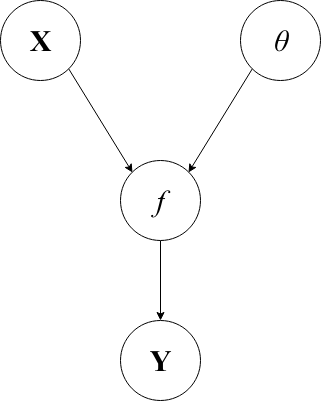
\includegraphics[width=0.5\linewidth]{question_10.png}}
\caption{Graphical model of the joint distribution.}
\label{fig:q10}
\end{figure}

The assumptions that have been made are:

\begin{itemize}
\item $\mathbf{X}$ and $\theta$ do not depend on anything;
\item $f$ depends on $\theta$ and $\mathbf{X}$;
\item $\mathbf{Y}$ depends on $f$, but is is conditionally independent of $\mathbf{X}$ and $\theta$.
\end{itemize}

\subsubsection*{Question 11}

The marginalisation $p(\mathbf{Y|X,\theta})$ connects the prior and the data because we now have a way to directly generate $\mathbf{Y}$ values given $\mathbf{X}$ and $\theta$ values without knowing the actual form of $f$.
\par
Because we are uncertain about $f$, when we marginalise it out, the uncertainty gets pushed onto $\mathbf{Y}$.
\par
The fact that $\mathbf{\theta}$ is left on the left hand side of the expression after marginalisation means that it is needed, along with $\mathbf{x}$, to calculate $\mathbf{Y}$. This implies that $\mathbf{Y}$ is dependent on theta.

\begin{figure}[htbp]
\centerline{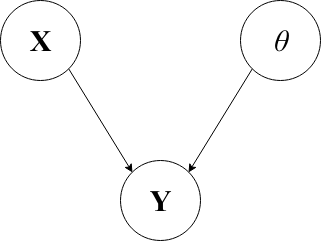
\includegraphics[width=0.5\linewidth]{question_11.png}}
\caption{Graphical model of the marginalised distribution.}
\label{fig:q11}
\end{figure}

The graphical model of the marginal $p(\mathbf{Y|X,\theta})$ is shown in Figure \ref{fig:q11} and shows how $\mathbf{Y}$ is now dependent on only $\mathbf{X}$ and $\mathbf{\theta}$.  The function $f$ (and its uncertainty) has been "baked in" to $\mathbf{Y}$.

%Use the model diagram to help?
%Marginalisation is the average of some distributions
%It is a weighted average of some functions, based on how likely each function is
\subsection{Practical}
\subsubsection{Linear Regression}
\subsubsection*{Question 12.1}

The prior distribution over $\mathbf{W}$ can be seen in the middle column of the top row of Figure \ref{fig:q12}. The red cross represents the true value of $\mathbf{W}$. The spherical covariance gives rise to a symmetrical distribution.

The rightmost column of the top row of Figure \ref{fig:q12} shows six random samples drawn from the prior which clearly do not have any well defined direction, which is exactly as expected since we have no data to make predictions with.

\subsubsection*{Question 12.2}

The second row of Figure \ref{fig:q12} show the result of picking a single data point. The leftmost column plots the likelihood distribution in $\mathbf{W}$-space of the data point. The middle column shows the posterior distribution after the likelihood has been combined with the prior. It can be seen visually that the prior has been squashed along the dimension of the likelihood. 

\subsubsection*{Question 12.3}

The rightmost column shows that the sampled functions now all pass through the observed data point, but do not yet agree completely in direction.

\subsubsection*{Question 12.4}

The lower two columns of Figure \ref{fig:q12} show the likelihood, posterior and data space samples after adding two and twenty points respectively. 

\begin{figure}[htb]
\centerline{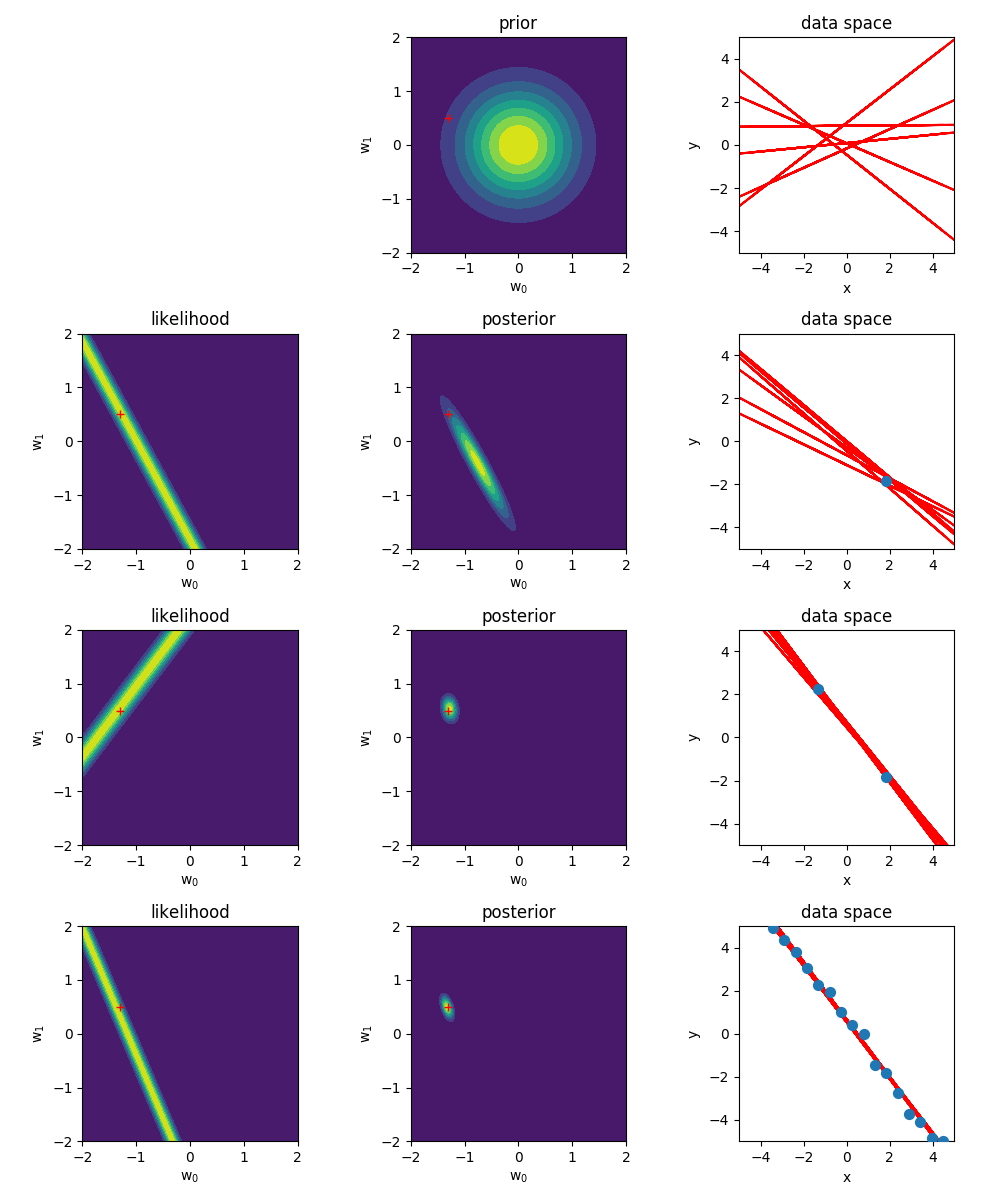
\includegraphics[width=\linewidth]{q12.png}}
\caption{Implementation of linear regression. The left hand column plots the likelihood. The middle column plots the prior/posterior, and the right hand column shows six random sample functions. Plots are drawn after one, two and twenty data points are revealed.}
\label{fig:q12}
\end{figure}

\subsubsection*{Question 12.5}
After a single data point is added, we can see that the posterior distribution begins to squash in one direction to converge onto the parameters $\mathbf{W}$. When we sample from this distribution, there are many lines passing through the point at different gradients, which is because we cannot define two parameters from a single data point. As we begin to reveal more data, the posterior distribution centres onto $\mathbf{W}$ and the sample functions fit more closely to the data points. This is exactly what we want to happen as it shows that we have relearned the parameters of the model used to generate the data $\mathbf{X}$.

\subsubsection*{Question 12.6}
The posterior converges on the position of $\mathbf{W}$ because after a new data point is added, we update the parameters using the newly calculated mean and covariance. As we see more data, we become more and more confident about the true value of $\mathbf{W}$.


\subsubsection{Non-parametric Regression}
\subsubsection*{Question 13}

Figure \ref{fig:q13} shows three examples of samples taken from a GP prior with a squared exponential covariance function that has a single hyper-parameter $l$ which encodes the length scale of the sample functions. The three values of $l$ are 0.1, 0.5 and 5 respectively.

\begin{figure}[htb]
\centering
\begin{subfigure}{.5\linewidth}
  \centering
  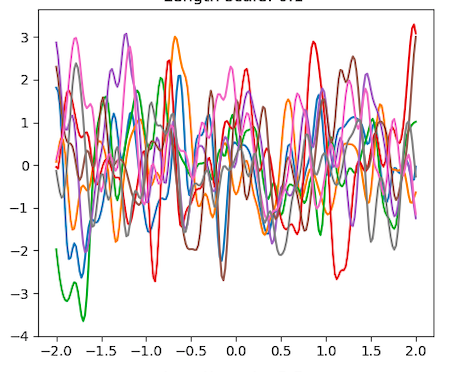
\includegraphics[width=.9\linewidth]{ls01.png}
  \caption{Length-scale of 0.1.}
  \label{fig:sub1}
\end{subfigure}%
\begin{subfigure}{.5\linewidth}
  \centering
  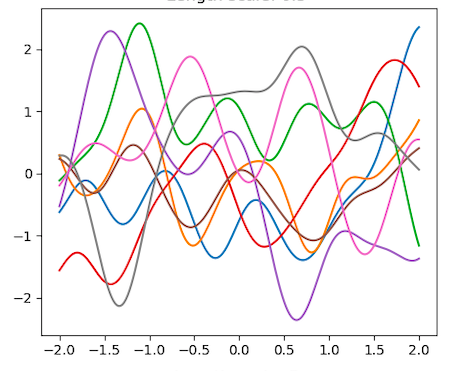
\includegraphics[width=.9\linewidth]{ls05.png}
  \caption{Length-scale of 0.5.}
  \label{fig:sub2}
\end{subfigure}
\begin{subfigure}{.5\linewidth}
\centering
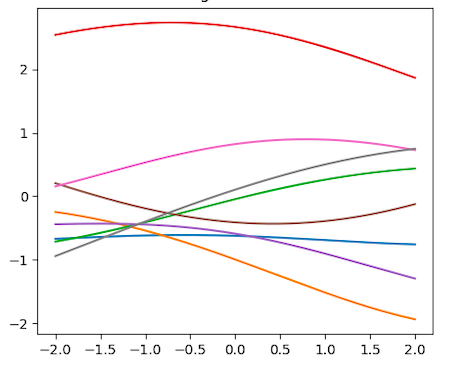
\includegraphics[width=0.9\linewidth]{ls5.png}
\caption{Length-scale of 5}
\end{subfigure}
\caption{Squared exponential with varying length scales. }
\label{fig:q13}
\end{figure}

Increasing the length-scale of the covariance function allows us to constrain the smoothness of the sample functions. A smaller length-scale creates functions with more rapid changes than those with a larger length-scale. This is because a higher length-scale means that, for two random variables $x_i$ and $x_j$ where the covariance is $k(x_i, x_j)$, their instantiations as $f_i$ and $f_j$ are similar. 

Choosing a larger length-scale encodes the assumption that smoother function with lower frequency is preferable to high frequency, more oscillatory functions. In other words, we prefer functions that change less rapidly.

\subsubsection{Question 14}

The predictive posterior distribution is a Gaussian given by 

\begin{align}
  p(\mathbf{Y}_{N+1}|\mathbf{Y}) = \mathcal{N}(\mathbf{M}_{N+1}, \mathbf{C}_{N+1})
\end{align}

where

\begin{equation}
  \mathbf{M}_{N+1} = \mathbf{k^T}\mathbf{C}_N^{-1}\mathbf{Y} \\
  \mathbf{C}_{N+1} = c - \mathbf{k^T}\mathbf{C}_N^{-1}\mathbf{k} 
\end{equation}

and $\mathbf{C_N}$ is the previous covariance matrix, $\mathbf{k}$ has elements $k(\mathbf{x}_n, \mathbf{x}_{N+1}$ (i.e. the kernel function invoked with all the previous data points and the new data point) and $c$ is a scalar that equals $k(\mathbf{x}_{N+1}, \mathbf{x}_{N+1}$ (i.e. the kernel function over just the new data point).

Need to describe the plots. What happens if we use a diagonal covariance matrix to the squared exponential. 

%functions not passing exactly through the data, do you have a diagonal term?
%If you look at slide 66 in lecture 6, if you set \sigma=0 then the functions
%should go straight through the data, if you have it larger than zero you have
%a "residual" variance that will be like a noise that can never be removed.

\begin{figure}[!htb]
\centerline{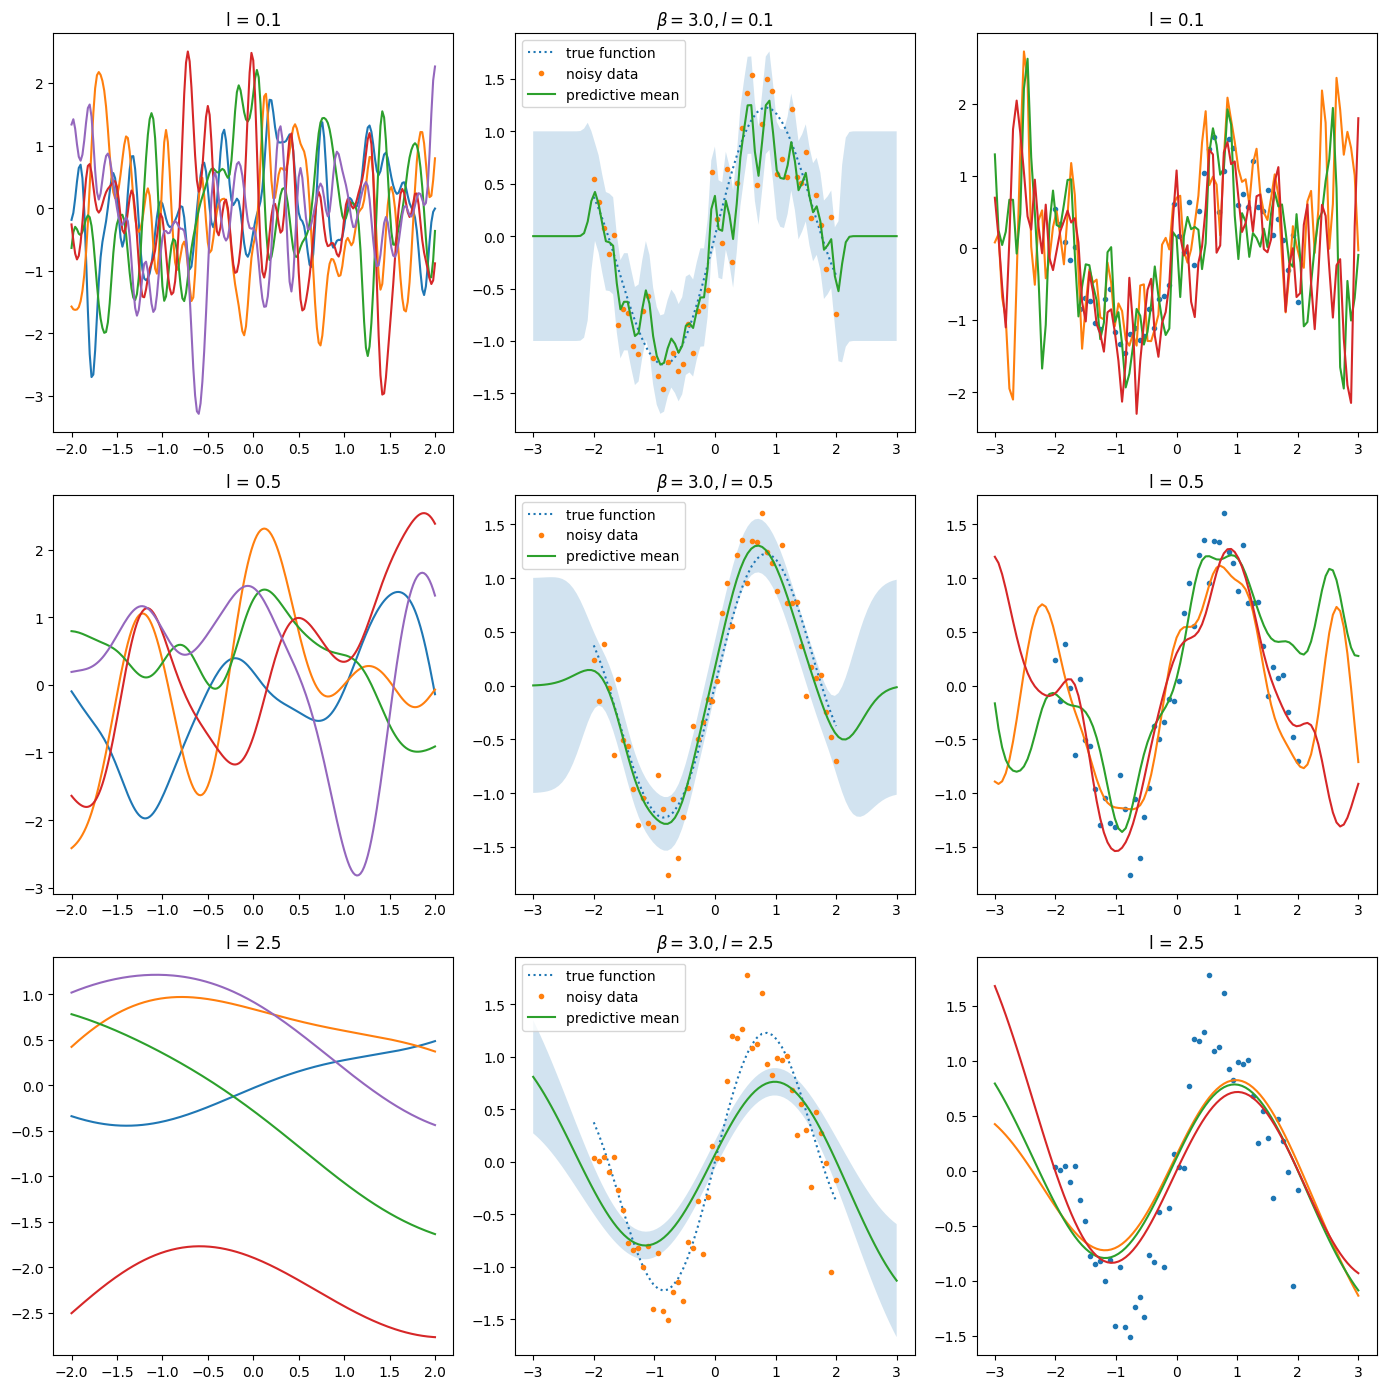
\includegraphics[width=\linewidth]{non_parametric_regression.png}}
\caption{Implementation of non-parametric regression with changing length-scales. }
\label{fig2}
\end{figure}

\section{Posterior}

\subsubsection*{Question 15}
We use our beliefs to find a starting point for the problem and to make assumptions about the data, or any other characteristics of the problem. Assumptions are what we assume to be true about something. If we had all the data we required for a problem, there would be no need to assume anything. This gives us a way to reason when we have very little information. \par
A preference is an assumption that we want to use because it is easier to do so. For example using a gaussian likelihood so that the posterior is also gaussian. -

We use beliefs and assumptions to formulate a prior. Believe that the smooth lines are more likely. Prefer straight or flat lines.

\subsubsection*{Question 16}

Since the covariance matrix is spherical, we have assumed that the latent input variables are independent and that they are centred around the origin. 

\subsubsection*{Question 17}

One way to obtain the marginal distribution $p(\mathbf{Y|W})$ would be to write out the exponents of the likelihood and the prior and do a lot of algebra to work out the actual integral. But there is a simpler way.

Firstly, we know that $\mathbf{Y = WX + \epsilon}$ and we know that $\mathbf{X}$ is Gaussian since we put a prior over it. We know that we can do any linear transformation to a Gaussian and it is still a Gaussian because Gaussians are closed under linear transformation. So we know that $p(\mathbf{Y|W})$ is going to be a gaussian. All we need to do is work out the mean and the covariance of the distribution we are looking for.

We know that the mean is the expectation of $\mathbf{Y}$, so we can therefore write

\begin{align} \label{eq:6}
  \mathbb{E}[\mathbf{Y}] = \mathbb{E}[\mathbf{WX} + \epsilon].
\end{align}

We know the expected value of $\mathbf{X}$ since we picked a prior over $\mathbf{X}$ and gave it a zero mean, so ti will be zero. We can also ignore $\epsilon$ in the expectation since it is just a noise parameter. Therefore we can deduce that the mean $\mu$ is just going to be zero.

Now to work out the covariance, we know that it is going to be the expected value of $\mathbf{Y}$ multiplied by its transpose, which we can write similarly to (\ref{eq:6}) as

\begin{align}
  \mathbb{E}[\mathbf{YY^T}] = \mathbb{E}[\mathbf{(WX + \epsilon)(WX + \epsilon)^T}] \\
  = \mathbb{E}[\mathbf{WXX^TW^T}] + \mathbb{E}[\mathbf{\epsilon\epsilon^T}]
\end{align}

The expectation of the noise parameter $\epsilon$ we have already defined as being $\sigma^2\mathbf{I}$. Since our prior over $\mathbf{X}$ was zero-mean, we know that $\mathbf{XX^T}$ is going to be the identity matrix, therefore can simply write the covariance as

\begin{align}
  \mathbb{E}[\mathbf{Y}] = \mathbf{WW^T + \sigma^2I}
\end{align}

which gives us the resulting marginal distribution

\begin{align}
  p(\mathbf{Y|W}) = \mathcal{N}(0, \mathbf{WW^T + \sigma^2I})
\end{align}

and we are done.

\subsubsection*{Question 18.1}
A maximum-a-posteriori (MAP) estimation is equal to the mode of the posterior. It finds the parameters that maximise the posterior distribution. Because it takes the posterior into account, it is a more computationally expensive operation. \par
The maximum likelihood (ML) can be seen as a type of MAP estimation, which assumes a uniform prior distribution of the parameters. In doing so, it finds the parameters that maximise the likelihood. \par
Type-II Maximum likelihood finds the parameters that maximise the marginal likelihood. 

%The prior is included in MAP, while ML only includes the likelihood. MAP takes both prior and likelihood into account.
%https://wiseodd.github.io/techblog/2017/01/01/mle-vs-map/

\subsubsection*{Question 18.2}
With only one data point, ML will be less accurate than MAP since it does not take the prior into account. However as more data is seen, the two will begin to converge on one another. 

\subsubsection*{Question 18.3}
The denominator of the posterior distribution has no bearing on the result as it will always be positive, and depends on the parameters $\mathbf{W}$. 

\subsubsection*{Question 19}

The objective function can be written as:

\begin{multline}
  \mathcal{L}(\mathbf{W}) = -log(p(\mathbf{Y}|\mathbf{W}, \bm{\mu}, \bm{\sigma}^2)) \\
  = -\frac{ND}{2}log(2\pi) - \frac{N}{2}log|\mathbf{C}| - tr(\mathbf{(YC)^{-1}Y^T})
\end{multline}

where $\mathbf{C} = \mathbf{WW^T} + \bm{\sigma^2}\mathbf{I}$. The gradients of the objective function with respect to the parameters can be written as:

\begin{multline}
  \frac{\partial \mathcal{L}}{\partial \mathbf{W}} = tr(\mathbf{C^{-1}(WJ_{ij} +  J_{ji}W^T)}) \\
  + tr(\mathbf{Y^TY(-C^{-1}(WJ_{ij} +  J_{ji}W^T)C^{-1}})
\end{multline}

where $\mathbf{WJ_{ij} +  J_{ji}W^T}$ = $\frac{\partial \mathbf{C}}{\partial \mathbf{W_{ij}}}$.

\subsubsection*{Question 20}
The uncertainty in $\mathbf{X}$ and $\theta$ is pushed into $f$. Therefore, by marginalising out $\mathbf{X}$, we lose some of the information required to calculate an accurate $\mathbf{Y}$.

\subsubsection*{Question 21}

We first mapped the input variables $\mathbf{x}$ non-linearly to a 2D space and plotted the result. This gives a uniform spiral shape as seen in Figure \ref{fig:sub1}. We then mapped this linearly to a 10D space. Given the objective function and gradients from above, we then minimised the log likelihood to "learn" the linear mapping parameters W. Using the new parameters, we performed the reverse of the linear mapping back to 2D space and obtained another (slightly different) spiral which can be seen in Figure \ref{fig:q21b}.

\begin{figure}[!htb]
\centering
\begin{subfigure}{.5\linewidth}
  \centering
  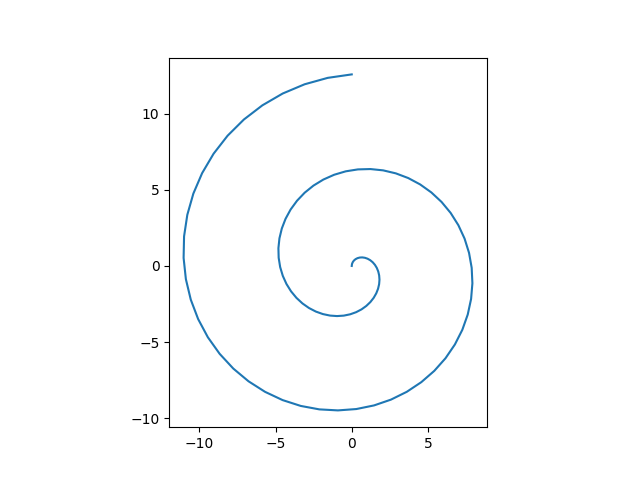
\includegraphics[width=.9\linewidth]{q21_a.png}
  \caption{Original 2D subspace.}
  \label{fig:q21a}
\end{subfigure}%
\begin{subfigure}{.5\linewidth}
  \centering
  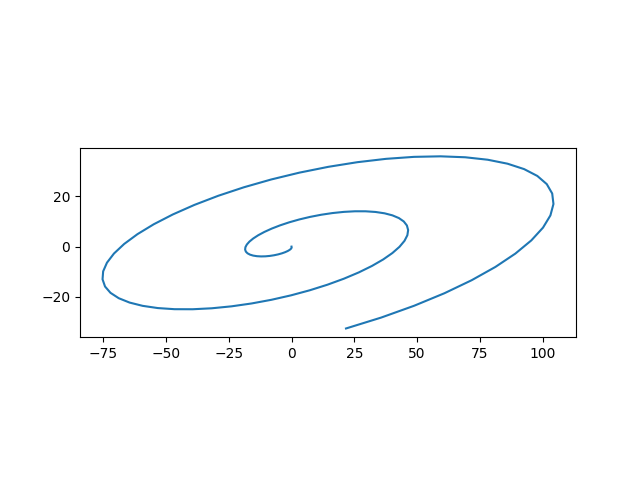
\includegraphics[width=.9\linewidth]{q21_b.png}
  \caption{Subspace learnt via Type-II ML.}
  \label{fig:q21b}
\end{subfigure}
\begin{subfigure}{.5\linewidth}
  \centering
  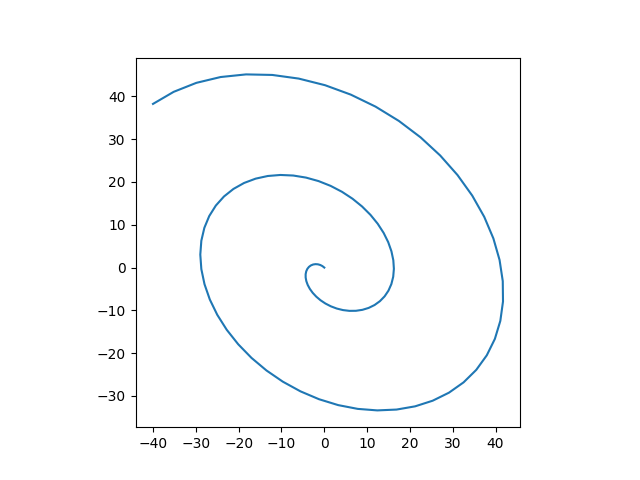
\includegraphics[width=.9\linewidth]{q22.png}
  \caption{Random subspace.}
  \label{fig:q22}
\end{subfigure}
\caption{Subspaces representing a 2D non-linear mapping from a 1D input vector. }
\end{figure}

We expected the recovered shape to be more similar to the original shape. We suspect there may be an error in the minimisation process (probably somewhere in computing the gradients).

Since we have only learned the parameters for the linear part of the mapping, it does not immediately appear possible to recover the original latent variables themselves.

\subsubsection*{Question 22}

Choosing any randomly initialised W matrix and performing the reverse mapping also results in a spiral shape, as can be seen in Figure \ref{fig:q22}. However, the shape is slightly different, the dimensions are different.


\section{The Evidence}

\subsubsection*{Question 23}

\subsubsection*{Question 24}

\subsubsection*{Question 25}

\section{Final Thoughts}
\subsubsection*{Question 30}
I feel that the purpose of this assignment was to introduce the basics of machine learning using a statistical, low level approach. In doing this, we have been forced to learn the theory behind algorithms before we are able to implement them. 
\par
The main learning point of this assignment has been the methodology of machine learning, which involves defining a prior and likelihood with the goal of finding a posterior distribution. 

%----------------------------------------------------------------------------------------
%	BIBLIOGRAPHY
%----------------------------------------------------------------------------------------

\printbibliography[title={Bibliography}] % Print the bibliography, section title in curly brackets

%----------------------------------------------------------------------------------------

\end{document}
